\documentclass{article}
\usepackage{amssymb}
\usepackage{amsthm}
\usepackage{amsfonts}
\usepackage{amsmath}
\usepackage{multirow}
\usepackage{enumitem}
\usepackage{gensymb}
\usepackage{graphics}
\usepackage{graphicx}
\usepackage{float}
\usepackage{hyperref}
\usepackage{caption}
\usepackage{biblatex}
\addbibresource{references.bib}

\hypersetup{
    colorlinks=true,
    linkcolor=blue,
    citecolor=cyan,
    urlcolor=cyan
    }

\setlength{\oddsidemargin}{-0.15in}
\setlength{\topmargin}{-0.5in}
\setlength{\textwidth}{6.5in}
\setlength{\textheight}{9in}
\allowdisplaybreaks

\title{TOCQ: Tackle Opportunity Containment Quotient in the 2022 National Football League Season (Weeks 1-9) \\ \small \quad \\
 \large Duke University Masters of Statistical Science Portfolio Report}
\author{Eli Gnesin}
\date{April 5, 2024}

\begin{document}

\maketitle

\section{Introduction and Motivation}

During a play in a football game, such as in the National Football League (NFL), the primary goal of the defenders is to stop the ball carrier from advancing. This can be by tackle, out of bounds, forcing a fumble, or forcing a slide. The box score, however, only credits the player(s) who actually ``make the tackle", as if they did so alone. A player who is often in the ``right place" but who is not credited for the tackle receives no credit for being ``in the right place at the right time". Conversely, a player who sees tackle ``opportunities" slip away does not see negative impact for it in the box score. With this in mind, I define \textbf{TOCQ}, or \textbf{Tackle Opportunity Containment Quotient}, which reflects a defender's ability to ``contain" the ``tackle opportunities" with which he interacts. I will first define \textbf{TOCQ} and explain the calculation process before discussing \textbf{TOCQ} in the first half of the 2022 NFL Season, using data provided during the 2024 NFL Big Data Bowl \cite{big_data_bowl}.

\section{Defining TOCQ}

\textbf{TOCQ} is the quotient of ``tackles contained" and ``tackle opportunities." Consider a defender $X$. The \textit{tackle zone} of defender $X$ is the sector of a circle, centered on the player with radius $r = \max(1.25, 1.25 + \frac{s}{10} + \frac{1}{2*100}a)\ yards$, with a $150^{\circ}$ sector angle bisected by a vector in defender $X$'s orientation direction. The reasoning behind this radius is that, in this range, it is feasible the defender, facing the ball, could both see and react to the ball carrier. Given NFL speeds rarely exceed 22 mph or $\sim 10.5$ yards/second, and a frame rate of 10 frames per second (fps), most players would take $\approx 3$ frames to pass through a tackle zone if completely unencumbered, at top speed, and the defender were static \cite{Sutelan_2023}. Further, if a player is moving forward, the tackle zone is adjusted by the displacement he would have before the next frame, using the standard displacement formula $\Delta x = st + \frac{1}{2}at^2$ for speed $s$ in yards per second, acceleration $a$ in yards per second squared, and time $t$, in order to recognize that the defender has increased range if he is moving in the direction of the ball as opposed to being static. Since the frame rate is 10 fps, the displacement formula is evaluated at $t = 0.1$, which gives the above radius calculation.

Now, consider an arbitrary play. For each frame between the ball snap + 2 frames (for run plays, adjusted to avoid unfairly penalizing defensive linemen who line up over the ball) or the pass completion (for pass plays), first calculate each defender's tackle zone, and then check if the football is inside the zone. If this is true for defender $X$, he is credited with a \textit{tackle opportunity}. Importantly, tackle opportunities are binary in a given play; even if the ball carrier leaves the tackle zone and later returns to it, he receives one tackle opportunity. When a play ends, whether by tackle, fumble, sack, slide, or out of bounds, that frame is the ``action frame," which is used to count ``tackles contained." If the ball is within a defenders's tackle zone during this frame, the defender is credited with a \textit{tackle contained}. How that involvement occurs is ignored; ``tackler" is the same as all other players with the ball in their zones. Any tackle contained is also simultaneously a tackle opportunity. 

For defender $X$, there are three outcomes:
\begin{enumerate}
    \item Defender $X$ has no \textit{tackle opportunity}. This is neutral for \textbf{TOCQ}.
    \item Defender $X$ has a \textit{tackle opportunity} but no \textit{contained tackle}. This is negative for \textbf{TOCQ}.
    \item Defender $X$ has a  \textit{tackle contained} and corresponding \textit{tackle opportunity}. This is positive for \textbf{TOCQ}.
\end{enumerate}

I now define \textbf{TOCQ$_X$} for defender $X$ as:

$$ TOCQ_X = \frac{\text{\# of Tackles Contained by Defender X}}{\text{\# of Tackle Opportunities for Defender X}} $$

Similarly, I define \textbf{TOCQ$_T$} for a team as:

$$ TOCQ_T = \frac{\text{\# of Tackles Contained by Team T}}{\text{\# of Tackle Opportunities for Team T}} $$

For consistency, \textbf{TOCQ} without a subscript refers to the general metric and the subscript is for disambiguation in discussing actual values between team and players. The two metric forms above have slightly different interpretations. For the individual player, a high \textbf{TOCQ$_X$} reflects a defender who ``makes the most of his opportunities" and is often ``in the right place at the right time." Conversely, a low \textbf{TOCQ$_X$} could reflect a defender who has opportunities pass but is not involved in as many plays. For a team, a high \textbf{TOCQ$_T$} reflects quick team containment of ball carriers and a lower \textbf{TOCQ$_T$} indicates a team which struggles to quickly contain ball carriers or has more ``hero" plays where one defender makes a play solo.

Consider an example play from the Week 2 game between the New York Jets (NYJ) and Cleveland Browns (CLE). Table \ref{table:ExamplePlay} shows an output table for the \textbf{TOCQ$_X$} scores for that single play. There are 11 rows, one for each of the 11 players on defense on that play. In this case, 4 players had a tackle opportunity, and 2 players had a containment, so they are denoted as such and every other player has a 0 in both column. Players are tracked across the season by an index of a unique player ID (provided in the dataset) and their team abbreviation.

\section{Sensitivity Analysis of Tackle Zone Radius and Standard Errors}

Before exploring the real outcomes for specific players and teams during the first half of the 2022 season, it is worth considering the sensitivity of \textbf{TOCQ} to the choice of tackle radius, as well as the standard error in the half-season \textbf{TOCQ$_X$} and game \textbf{TOCQ$_T$} scores. For this, I considered varying tackle radii of $r = max(c, c + st + \frac{1}{2}at^2)$ for $c = 1, 1.25, 1.5$ (where $c = 1.25$ was the value used for \textbf{TOCQ} in the analysis stage), denoted as "$c$yd Varying," as well as a constant radius $r = 1.5$, denoted as "$1.5$yd Constant," for comparison. Likewise, it is worth considering the density of half-season \textbf{TOCQ$_X$} scores and half-season tackle opportunity counts at these 4 radii, as well as the mean and standard error of the mean. For all 4 radii, there are 869 players with \textbf{TOCQ$_X$} scores, and 136 games, resulting in 272 \textbf{TOCQ$_T$} scores (since each game has a \textbf{TOCQ$_T$} score for each team).

First, looking at the densities in Figure \ref{fig:SensitivityAnalysisTOCQ}, the density of half-season \textbf{TOCQ$_X$} scores are relatively similar, with the smaller varying radius of $1.0$ yards being slightly left-shifted and the larger varying radius of $1.5$ yards being slightly right-shifted. All four radii show similar unimodal density with small clusters of data at both 0 and 1 due to players with small sample size (if a player had zero opportunities, he was also recorded as having \textbf{TOCQ$_X$} = 0). Looking at the densities of the tackle opportunities in Figure \ref{fig:SensitivityAnalysisN} reinforces Figure \ref{fig:SensitivityAnalysisTOCQ}; the smaller varying radius of $1.0$ yards has its density slightly more concentrated towards zero than the larger radii, and the larger radius of $1.5$ yards has a fatter right tail than the other radii. 

\begin{table}[H]
    \centering
    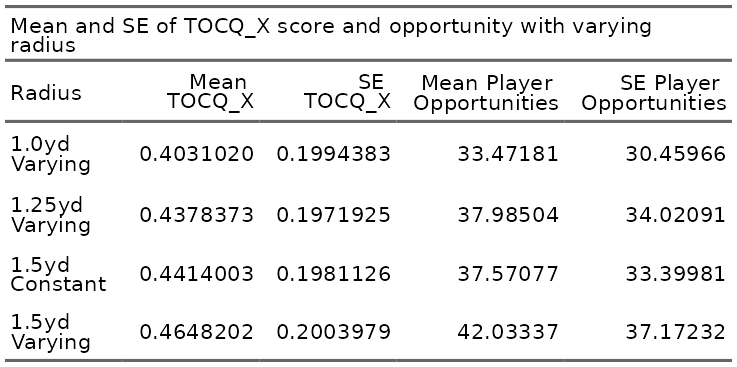
\includegraphics[width = .7\textwidth]{SensitivityTable.png}
    \caption{Table of mean and standard error of half-season \textbf{TOCQ$_X$} and tackle opportunities with varying tackle zone radius.}
    \label{table:SensitivityTable}
\end{table}

Looking at Table \ref{table:SensitivityTable} provides further support to the argument that the choice of tackle zone radius has minimal impact on the overall distribution of \textbf{TOCQ$_X$} scores. For all four radii, the mean, half-season \textbf{TOCQ$_X$} score is within $0.062$, which is significantly less than the standard error of all four radii, which hovers around $0.20$. Since \textbf{TOCQ} scores are bounded between 0 and 1, this is a large standard error, and suggests that there is no statistically significant difference between the means of the densities. Conversely, though there is a seemingly large difference in the mean number of opportunities based on the radius, with the 1.0 yard varying radius having a mean number of opportunities $\approx 8.5$ lower than the 1.5 yard varying radius, the standard error of all the opportunity counts is over 30, again indicating that there is not a statistically significant difference between the radii.

\begin{table}[H]
    \centering
    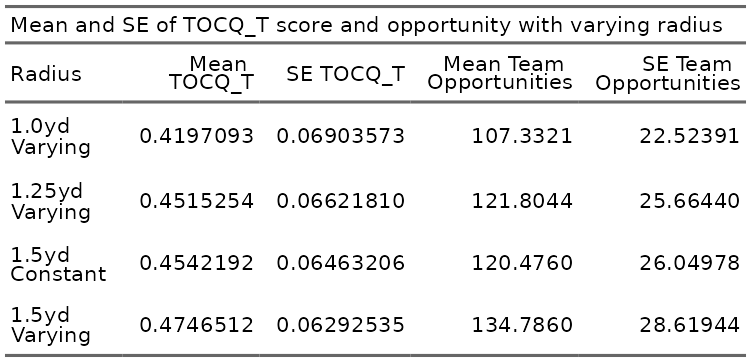
\includegraphics[width = .7\textwidth]{SensitivityTableTeam.png}
    \caption{Table of mean and standard error of team single game \textbf{TOCQ$_T$} and tackle opportunities with varying tackle zone radius.}
    \label{table:SensitivityTableTeam}
\end{table}

Similarly, it is worthwhile to compare the choice of tackle zone radius with respect to the team game \textbf{TOCQ$_T$} scores and the team number of opportunities per game, as presented in Table \ref{table:SensitivityTableTeam}. Due to the much larger sample size per game, even as opposed to an individual player over 8-9 games, the standard error of the \textbf{TOCQ$_T$} scores is much lower than the individual player level (there are no 0 or 1 values at the game level, and as noted in \ref{table:GameTeamScores} all single game \textbf{TOCQ$_T$} scores fall between 0.22 and 0.63). Further, with the mean team opportunities, there is again a positive correlation between the size of the varying radii and the mean team opportunities, though again the high standard error in both the \textbf{TOCQ$_T$} scores and the team opportunities indicates that these differences are not statistically significant.

The rest of the analysis proceeds with the 1.25 yard varying radius, that is $r = max(1.25, 1.25 + st + 0.5at)$. Since $TOCQ$ is explanatory, rather than predictive, there is no metric by which to measure a ``optimal" radius. As explained before, the 1.25 yard varying radius is intuitively driven given player speeds and a simple accounting of player motion, though further exploration of a ``optimal" radius is a potential future step.

\section{TOCQ for Weeks 1-9, 2022}

Using the metric defined in Section 2, as well as the radius established in Section 3, I calculated \textbf{TOCQ} for individual players and teams in the first half of the 2022 Season. There are 136 games and 869 players who played a defensive snap (including 4 offensive players). First, I calculated \textbf{TOCQ$_X$} for single games and for the half-season. To focus on regular players and to rule out players who may have only played a few plays or a single game, I am only presenting \textbf{TOCQ$_X$} scores for players with 30 or more opportunities for the half-season. Further, given the small sample size of any individual game, and acknowledging the large variance in even half-season scores in Figure \ref{fig:SensitivityAnalysisTOCQ}, single game scores for individual players are not considered, since no conclusions can be drawn from them.

Table \ref{table:HalfSeasonPlayer} shows the top 10 and bottom 10 players by half-season \textbf{TOCQ$_X$} score, of players with a minimum 30 opportunities, of which 442 players, or 50.9\%, qualify. The top 10 players by half-season \textbf{TOCQ$_X$} are mostly defensive backs, led by Pittsburgh Steelers Cornerback (CB) Levi Wallace. The bottom 10 players are all considered defensive linemen, with the exception of Za'Darius Smith of the Minnesota Vikings, who is marked as an Outside Linebacker but also regularly acts as a Defensive End. This is reasonable; on run plays, a defensive lineman, especially at the center of the line, can pick up a tackle opportunity if the running back cuts from one side of the line to the other, even if the defensive lineman is, himself, engaged with an offensive lineman as a blocker. Since tackle opportunities ignore blocker position, defensive linemen can pick up these ``phantom" opportunities when, though they are in range, actually containing the rusher is not nearly as clear-cut. Secondary players, conversely, likely only have opportunities when they are ``in on the play," and may often be the primary defender responsible on a pass play, which defensive linemen rarely are. 

With this in mind, I then considered the distribution of \textbf{TOCQ$_X$} scores (among players with 10 or more opportunities in the half season, of which 657 players, or 75.6\%, qualify) by position and position group. Figure \ref{fig:HalfSeasonPositionGroup} shows these distributions by boxplots by position, colored by the three ``position groups," defensive line, linebackers, and secondary. Figure \ref{fig:HalfSeasonPositionGroup} reinforces some of the trends seen in Table \ref{table:HalfSeasonPlayer}. Among position groups, secondary players mostly have higher mean \textbf{TOCQ$_X$} scores, while defensive linemen mostly have lower mean \textbf{TOCQ$_X$} scores. Acknowledging the large standard errors discussed in Table \ref{table:SensitivityTable}, and based on the boxplots of Figure \ref{fig:HalfSeasonPositionGroup}, however, no statistically significant conclusions can be drawn from these data.

I then move to consider \textbf{TOCQ} at the team level. As noted, \textbf{TOCQ} at the team level is denoted as \textbf{TOCQ$_T$}. As with \textbf{TOCQ$_X$} for individual players, \textbf{TOCQ$_T$} can be calculated for teams in single games and over the half-season. Unlike \textbf{TOCQ$_X$} above, \textbf{TOCQ$_T$} includes all players on each team in each game, since the calculation of \textbf{TOCQ$_T$} sums over all players, and small sample sizes are not an issue. As noted in Table \ref{table:SensitivityTableTeam}, the mean number of opportunities per game per team is over 120.

Table \ref{table:GameTeamScores} shows the top and bottom 10 games by \textbf{TOCQ$_T$} scores. As noted in Table \ref{table:SensitivityTableTeam}, \textbf{TOCQ$_T$} scores have much less variance than the \textbf{TOCQ$_X$} scores in table \ref{table:HalfSeasonPlayer}. Looking at Table \ref{table:GameTeamScores}, there are few patterns or trends, but the Carolina Panthers (CAR) has the 2 worst team performances in the dataset in weeks 5, and 7. Given Carolina was poor in 2022, this is unsurprising, and suggests their defense struggled to finish plays when they were close to ball carriers. On the flipside, the top 10 team games are represented by 10 different teams, and 4 teams appear on both lists in different weeks. Looking at Figure \ref{fig:HalfSeasonTeam} shows several different trends in the mean \textbf{TOCQ$_T$} scores by team. Carolina is far and away the worst team by \textbf{TOCQ$_T$} in the dataset, and appears to almost single-handedly drag the ``league average" below the league median. There are fewer noticeable trends in the teams than in the player \textbf{TOCQ$_X$} scores. The ``below average teams" include playoff teams such as the Dallas Cowboys (DAL), Jacksonville Jaguars (JAX), and Tampa Bay Buccaneers (TB), as well as the Houston Texans (HOU), and Chicago Bears (CHI), two of the three worst teams in 2022 \cite{Pro_Football_Reference}. The best team by \textbf{TOCQ$_T$} is the Minnesota Vikings (MIN), which went 8-1 in the dataset and made the playoffs, as well as the Super Bowl runner-up Philadelphia Eagles (PHI), and the Pittsburgh Steelers (PIT) and Detroit Lions (DET), both of which started the season poorly and then turned their seasons around in the second half of the season (outside the dataset) \cite{Pro_Football_Reference}.

Finally, Figure \ref{fig:HalfSeasonTeamPosGroup} shows the ratio of the average half-season \textbf{TOCQ$_T$} to league average in that position group, broken down into the three major position groups. This is a team level equivalent to Figure \ref{fig:HalfSeasonPositionGroup}, though it demonstrates which teams overperformed and underperformed league average. The struggles of Carolina are most apparent on this figure, given the bright red marks for their defensive line and linebackers, while Philadelphia stands out for their defensive line overperformance, which is unsurprising considering they were at the top of the NFL in Sacks and Total Defense during this span \cite{Stathead.com}. Overall, Figure \ref{fig:HalfSeasonTeamPosGroup} helps identify which position groups of teams are contributing most strongly positively or negatively towards the team scores seen in Figure \ref{fig:HalfSeasonTeam}, relative to the league average of those position groups.

\section{Conclusions, Limitations, Future Steps}

This paper introduces the metric \textbf{TOCQ: Tackle Opportunity Containment Quotient}, parameterized for both individual players and full teams. \textbf{TOCQ} also introduces the \textit{tackle zone}, the \textit{tackle opportunity} when the football enters the tackle zone, and the \textit{tackle containment} when the play ends within a defender's tackle zone. At the individual player level, defensive linemen, specifically defensive tackles, have generally lower \textbf{TOCQ$_X$} scores than linebackers and secondary players. At the team level, the top teams by \textbf{TOCQ$_T$} include several teams that underperformed early in the season, such as Pittsburgh and Detroit, as well as strong playoff teams in Minnesota and Philadelphia, and the lowest teams include several teams with middling records such as Carolina, Denver, and Cleveland.

There are several limitations to this analysis and \textbf{TOCQ} as currently presented. With the dataset provided, only nine weeks of games from a single NFL season are available. Though \texttt{plays.csv} contains approximately 12,500 plays, restricting to only these weeks puts many players under the number of opportunities I thought sufficient to draw conclusions from (I chose 30 as the traditional statistical threshold for ``small sample size"). As such, I chose not to analyze individual players from single game \textbf{TOCQ$_X$} scores, which would be a more granular level of analysis. This does not affect \textbf{TOCQ$_T$}, as noted, because a full game has a large enough sample of opportunities, but comparing teams on a sample of 8-9 games (depending on bye week) is also likely inadvisable due to the small sample size.

Within the dataset, I made several decisions which may have had adverse effects on the results. First, at least three plays were removed for missing player tracking data, and it is possible that are other plays have missing, incomplete, or incorrect player tracking data. More importantly, the choices I made regarding the frame events in the player tracking data may have significantly impacted the \textbf{TOCQ} scores. I chose to only consider frames between two frames after the ``ball snap" (on run plays) or from the ``pass outcome caught" frame (on pass plays) and through the tackle/out of bounds/slide/sack/fumble frame. I chose this because, for pass plays, not every frame from the ball snap is available, so I sought consistency. This, however, creates inconsistency between pass and run plays, which cannot be resolved because data from the snap is not provided on passing plays. Relatedly, while the decision to adjust to 2 frames after the snap does avoid penalizing defensive linemen for lining up over the snap (i.e. across from the center), the choice of 2 frames is heuristically chosen and may be improved upon. Further, there may be errors in the event tagging which would cause the incorrect frames to be used in individual plays and could, if numerous enough, impact the results.

With changing the \textbf{TOCQ} metric and definition or calculation of tackle zones and tackle opportunities in the future, while player speed and acceleration were accounted for in the tackle zone measurement, there may be more complex, elegant ways of measuring a player's motion to calculate an increased range. Further, the tackle zone is still based off a constant, $c = 1.25$, and it could be better to have that constant vary based on an individual player's attributes, such as wingspan or height. Likewise, as noted previously, exploring \textbf{TOCQ} in a predictive sense could lend itself towards an ``optimal" radius for each player, as measured by some convex function.

Finally, the tackle zone currently ignores the presence of blockers within the zone. This was deliberate; on many run plays, for example, an interior defensive lineman may be ``obstructed" by a blocker and still make a tackle, but this could be changed, and it is possible that this decision is part of the reason defensive linemen have lower \textbf{TOCQ} scores. \textbf{TOCQ} would, in this vein, benefit from a more consistent set of frames in each play, instead of separate between run and pass plays.

\printbibliography

\section{Appendix}

All code for calculating TOCQ and generating figures is found in \href{https://github.com/elignesin/Big-Data-Bowl-2024/}{this github repository}. Data is found at the Big Data Bowl link on \href{https://www.kaggle.com/competitions/nfl-big-data-bowl-2024/data}{Kaggle}.

\subsection{Figures and Tables}

\begin{table}[H]
    \centering
    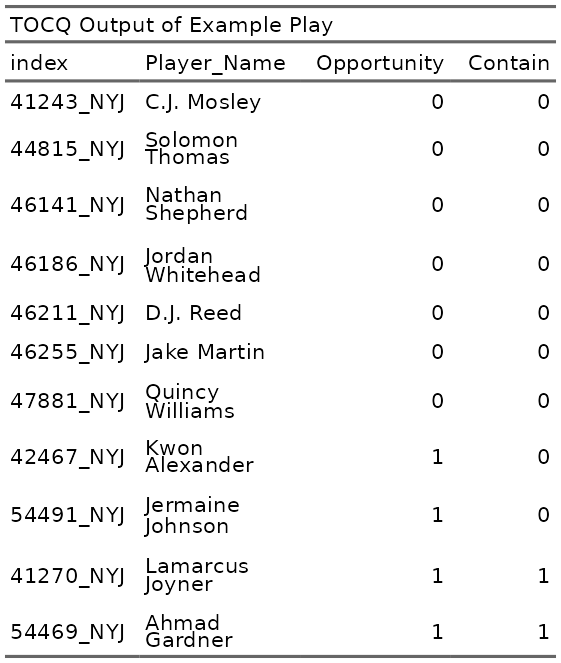
\includegraphics[width=0.5\textwidth]{ExamplePlay.png}
    \caption{\textbf{TOCQ} for a single play.}
    \label{table:ExamplePlay}
\end{table}

\begin{figure}[H]
    \centering
    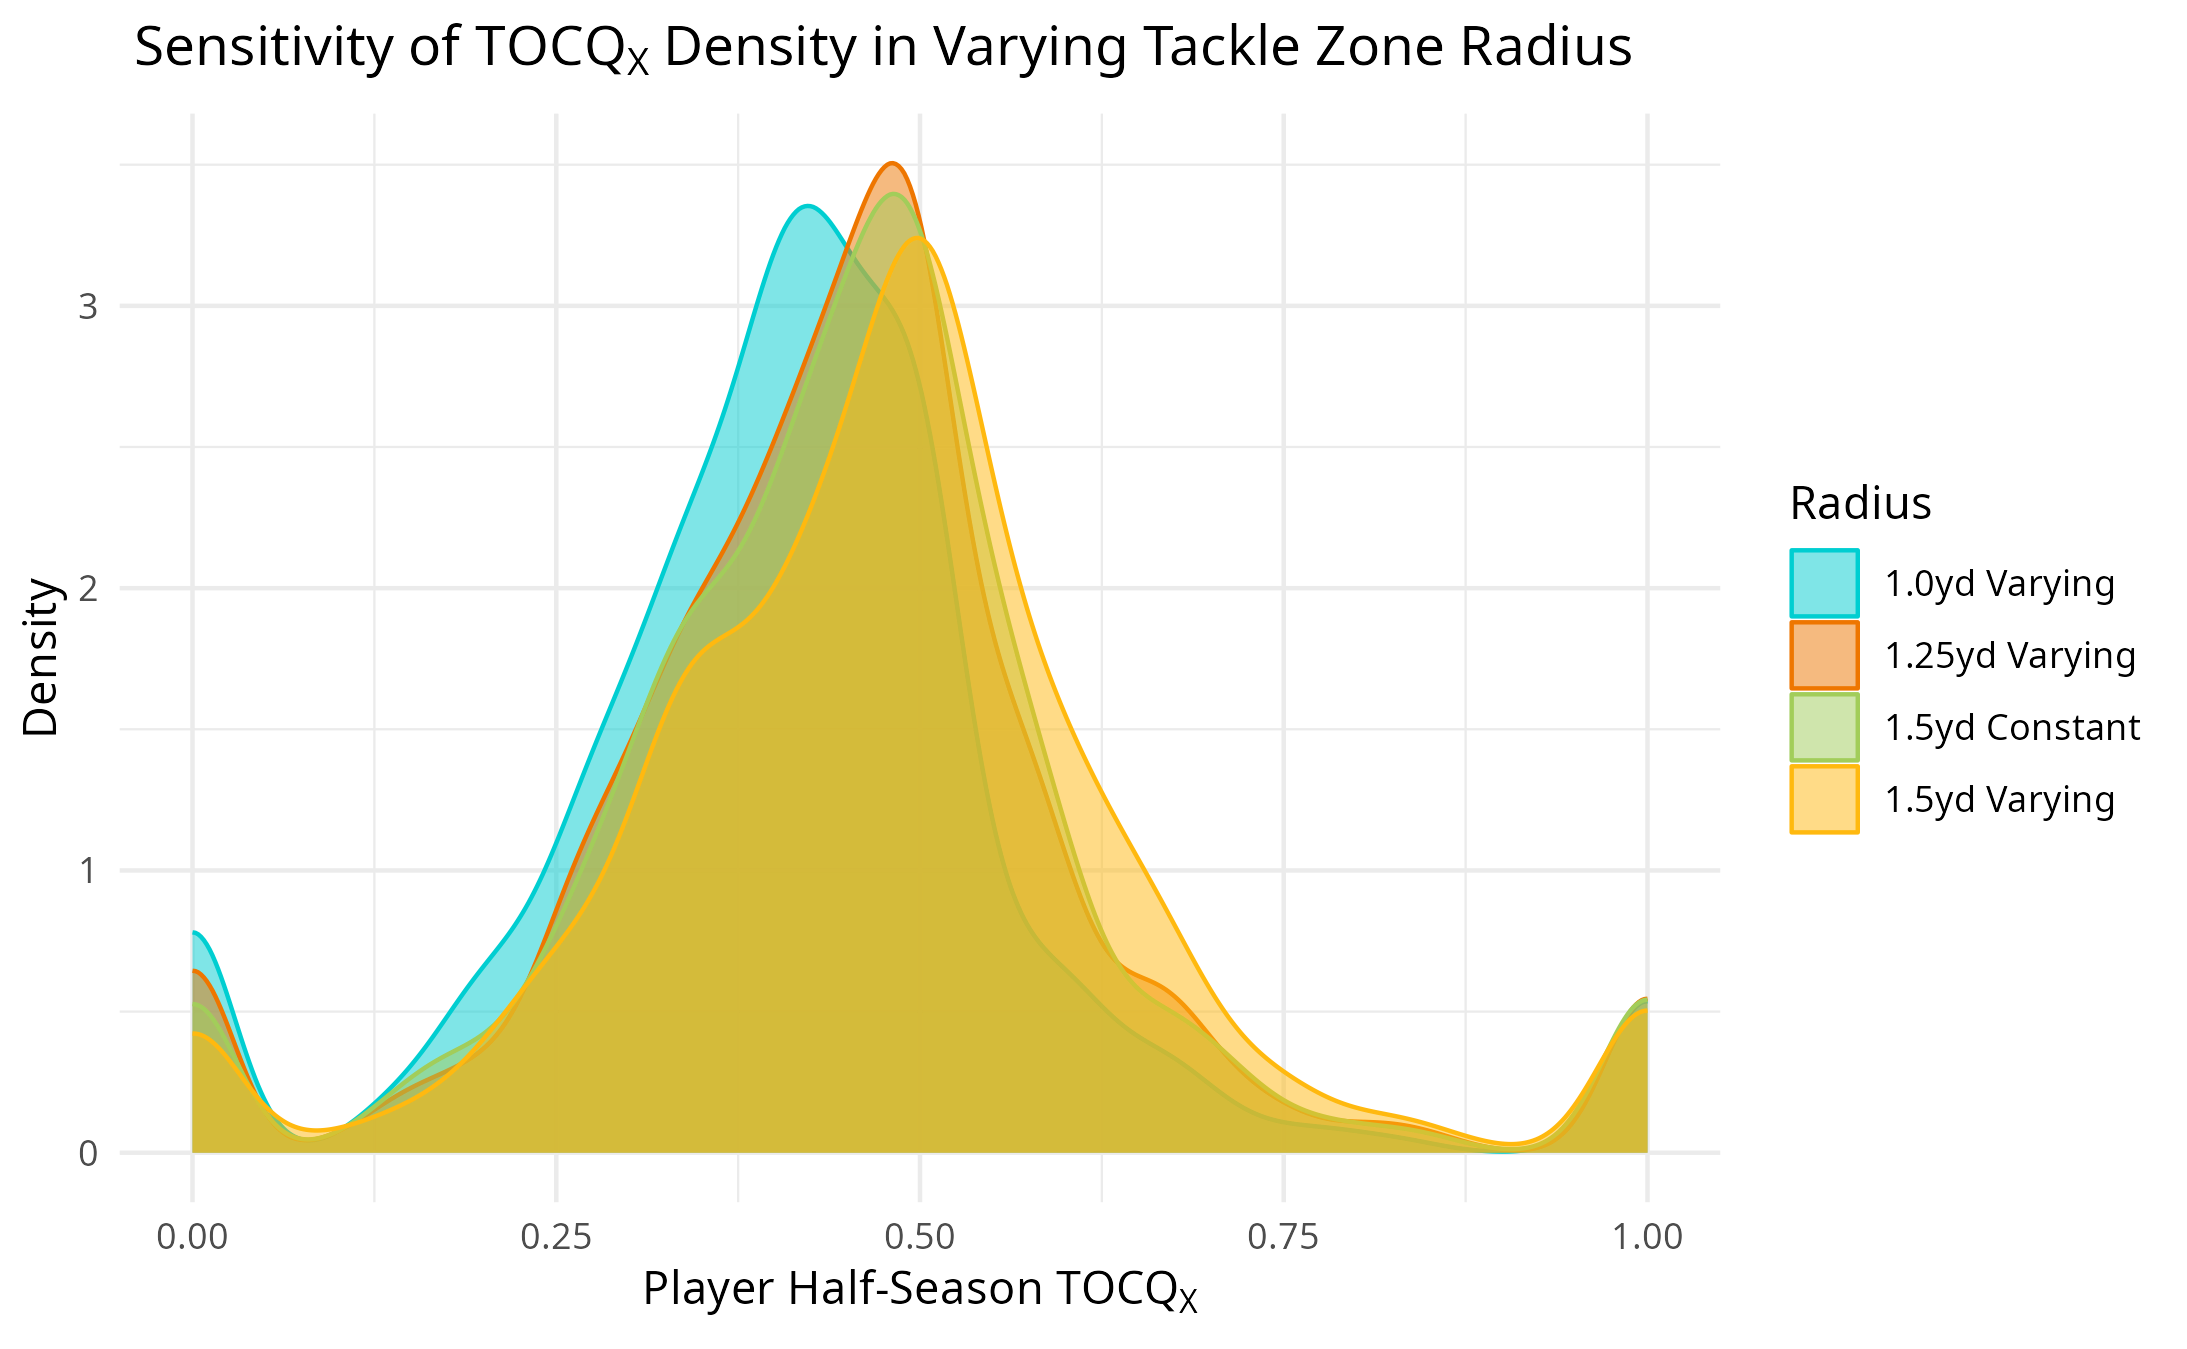
\includegraphics[width = \textwidth]{SensitivityAnalysisTOCQ.png}
    \caption{Density of half-season \textbf{TOCQ$_X$} scores with varying tackle zone radius.}
    \label{fig:SensitivityAnalysisTOCQ}
\end{figure}

\begin{figure}[H]
    \centering
    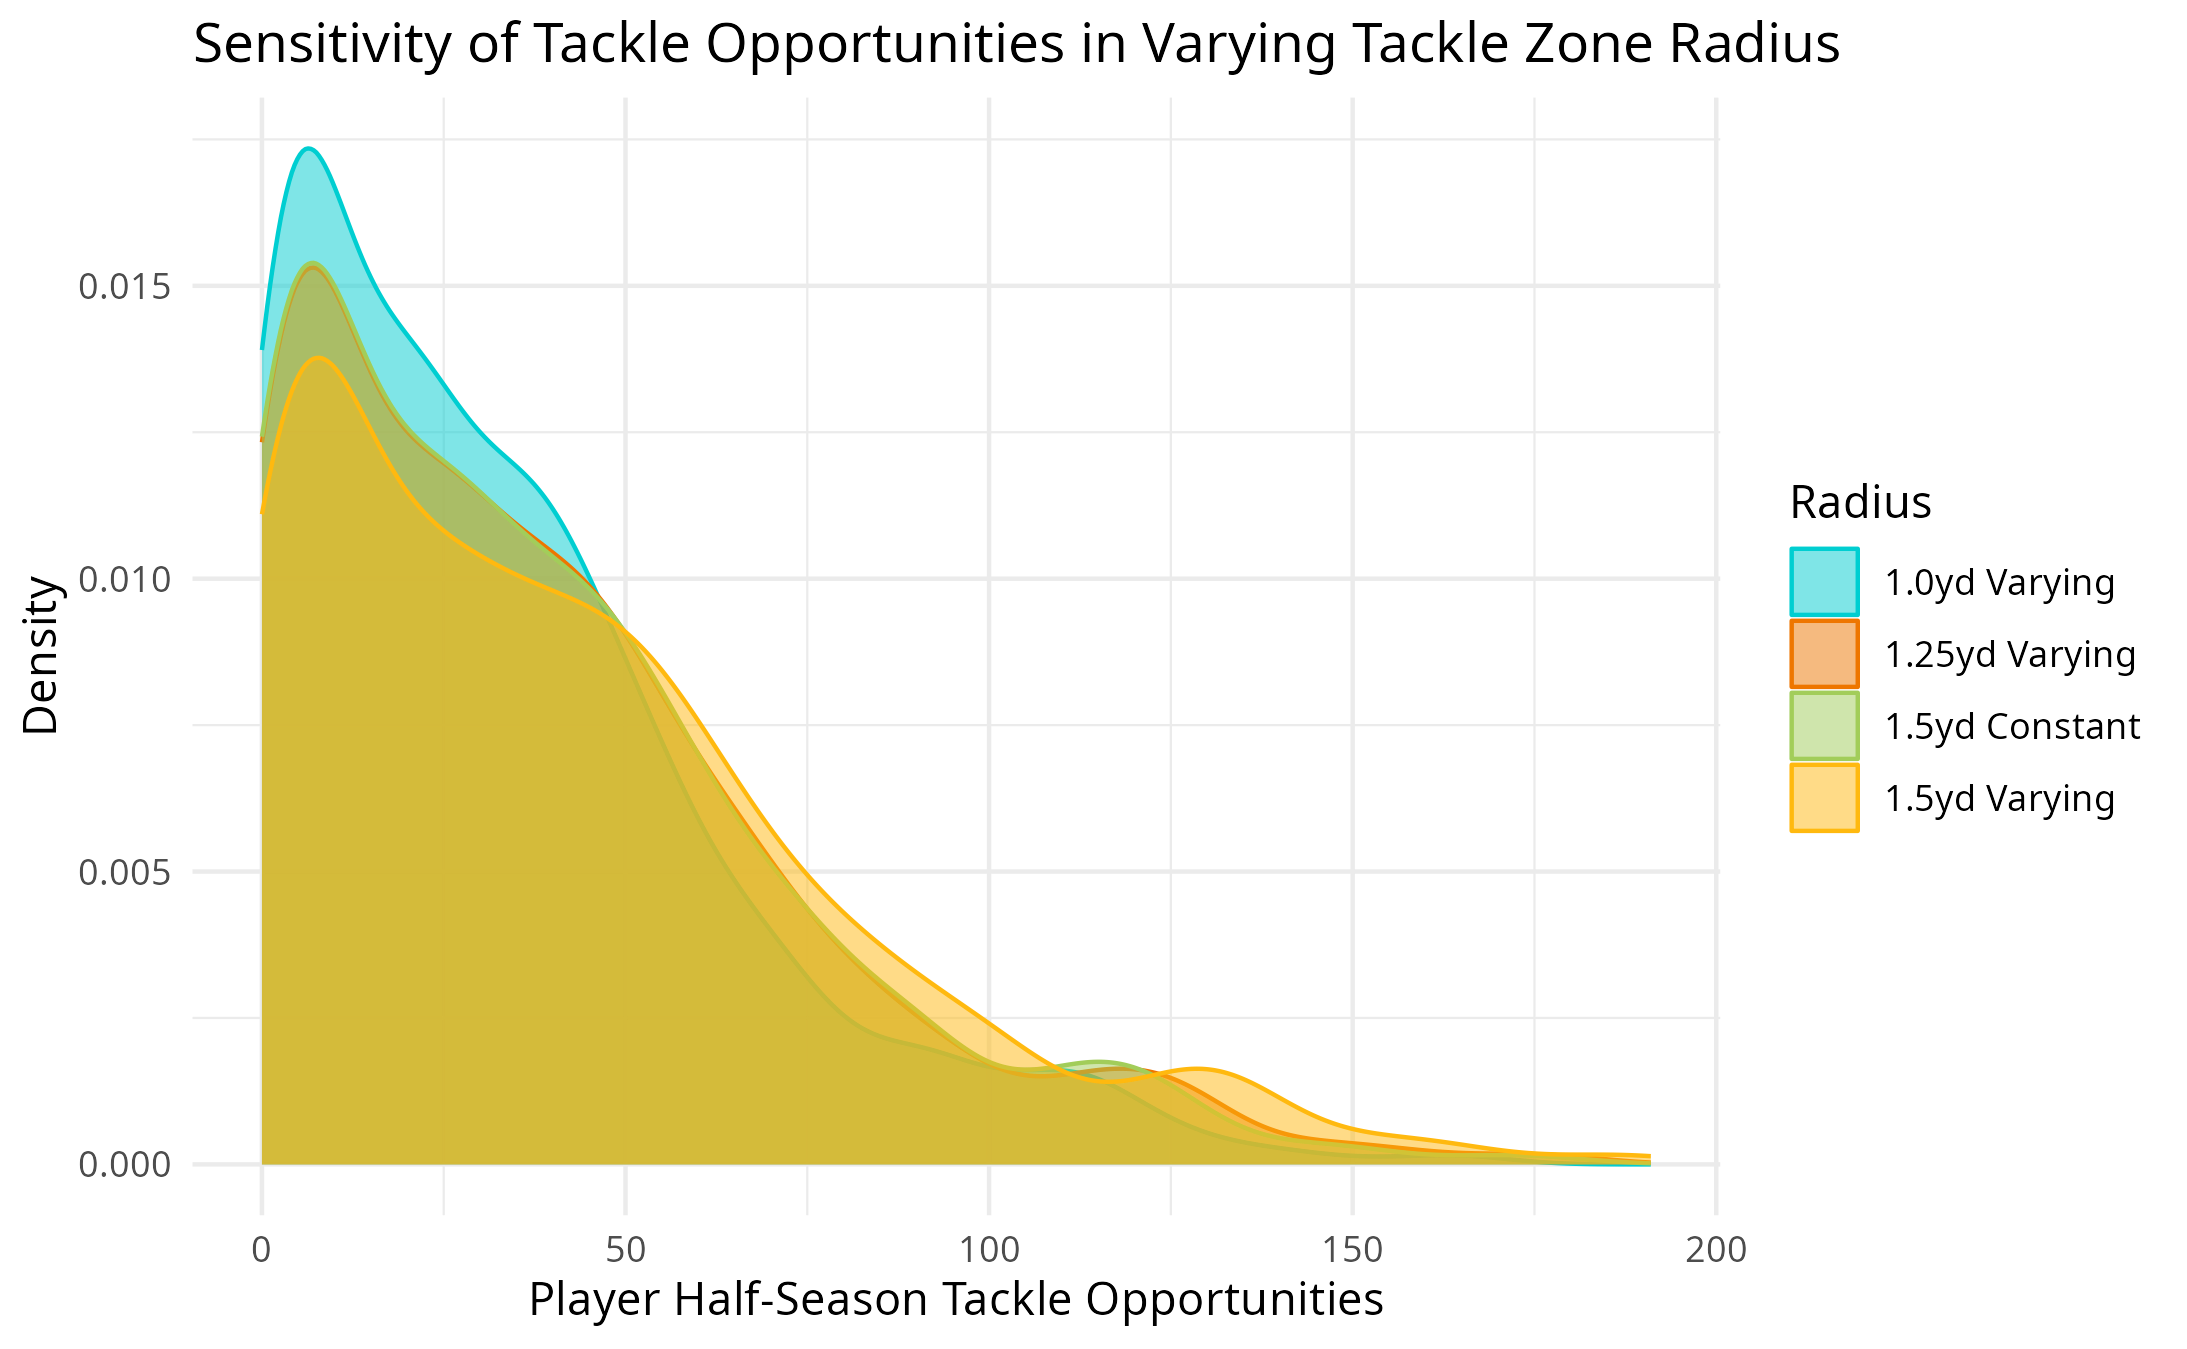
\includegraphics[width = \textwidth]{SensitivityAnalysisN.png}
    \caption{Density of half-season player tackle opportunities with varying tackle zone radius.}
    \label{fig:SensitivityAnalysisN}
\end{figure}

\begin{table}[H]
    \centering
    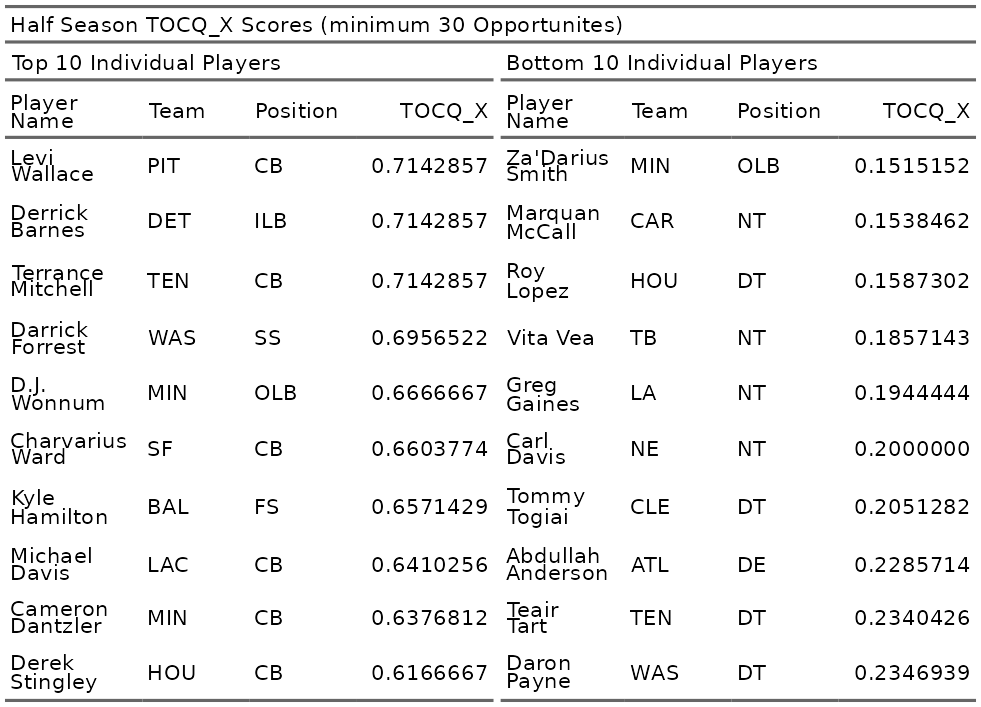
\includegraphics[width = \textwidth]{HalfSeasonPlayerScores.png}
    \caption{Player \textbf{TOCQ$_X$} scores for the half-season.}
    \label{table:HalfSeasonPlayer}
\end{table}

\begin{figure}[H]
    \centering
    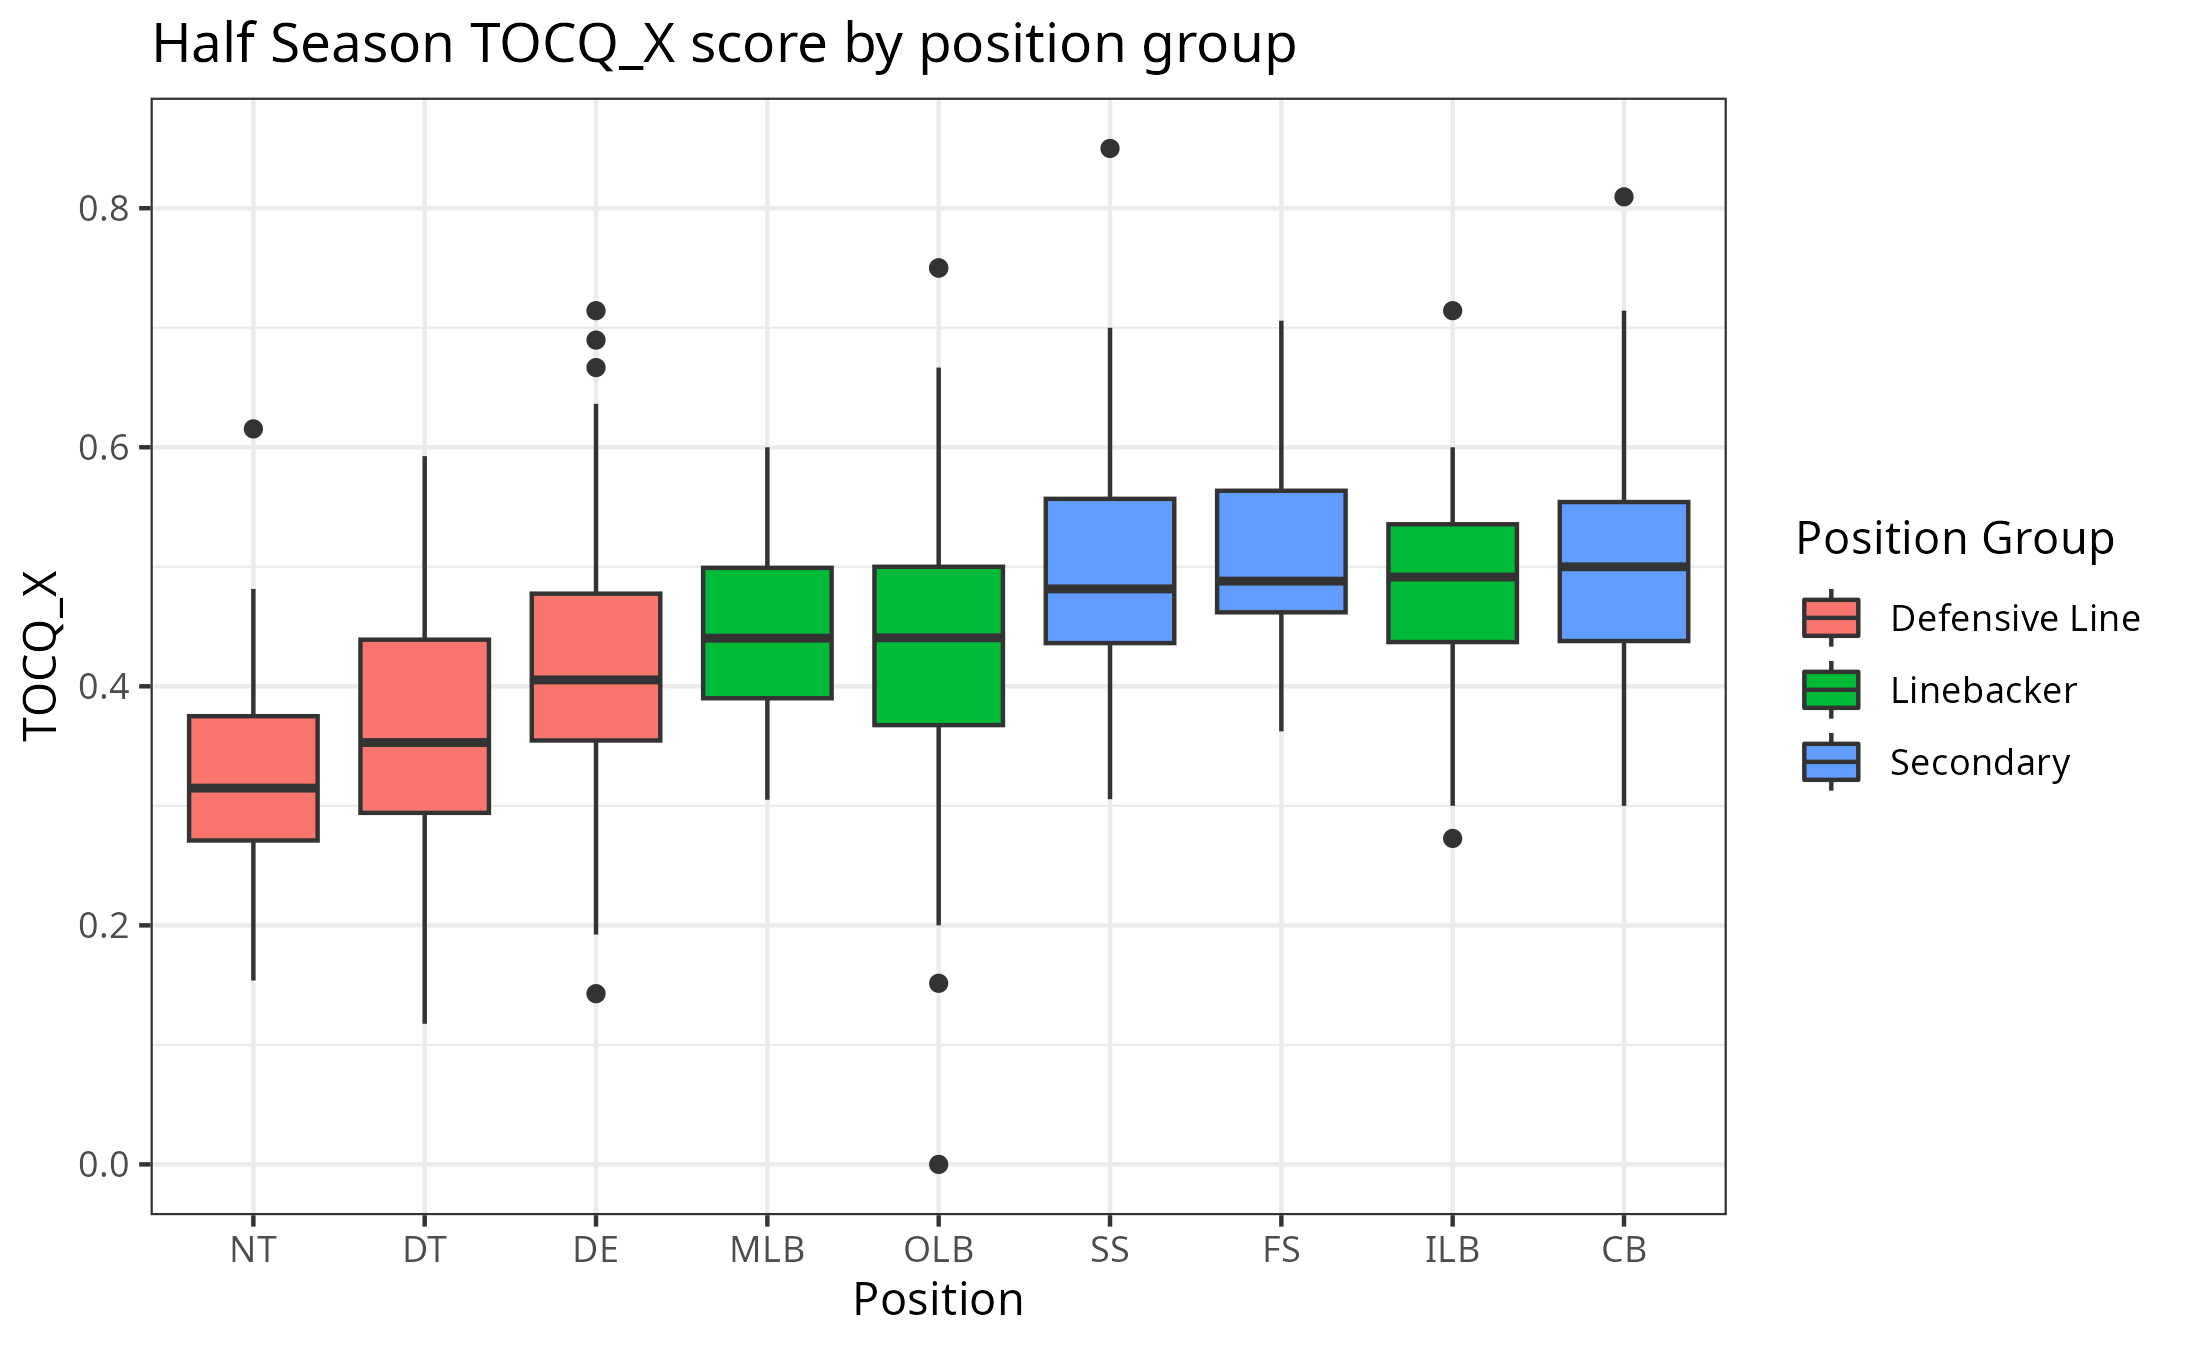
\includegraphics[width = \textwidth]{HalfSeasonPositionGroup.png}
    \caption{Distribution of half-season \textbf{TOCQ$_X$} scores by position group.}
    \label{fig:HalfSeasonPositionGroup}
\end{figure}

\begin{table}[H]
    \centering
    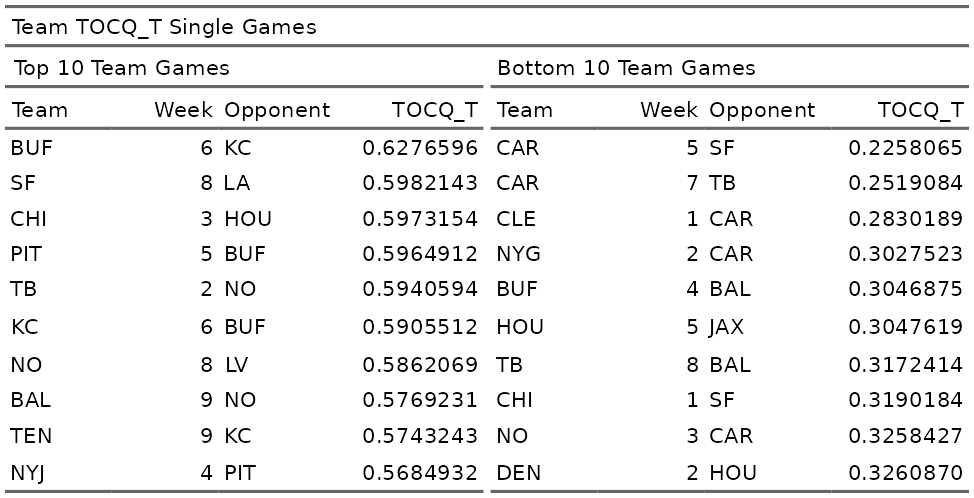
\includegraphics[width = \textwidth]{GameTeamScores.png}
    \caption{Best and worst single game team \textbf{TOCQ$_T$} scores.}
    \label{table:GameTeamScores}
\end{table}

\begin{figure}[H]
    \centering
    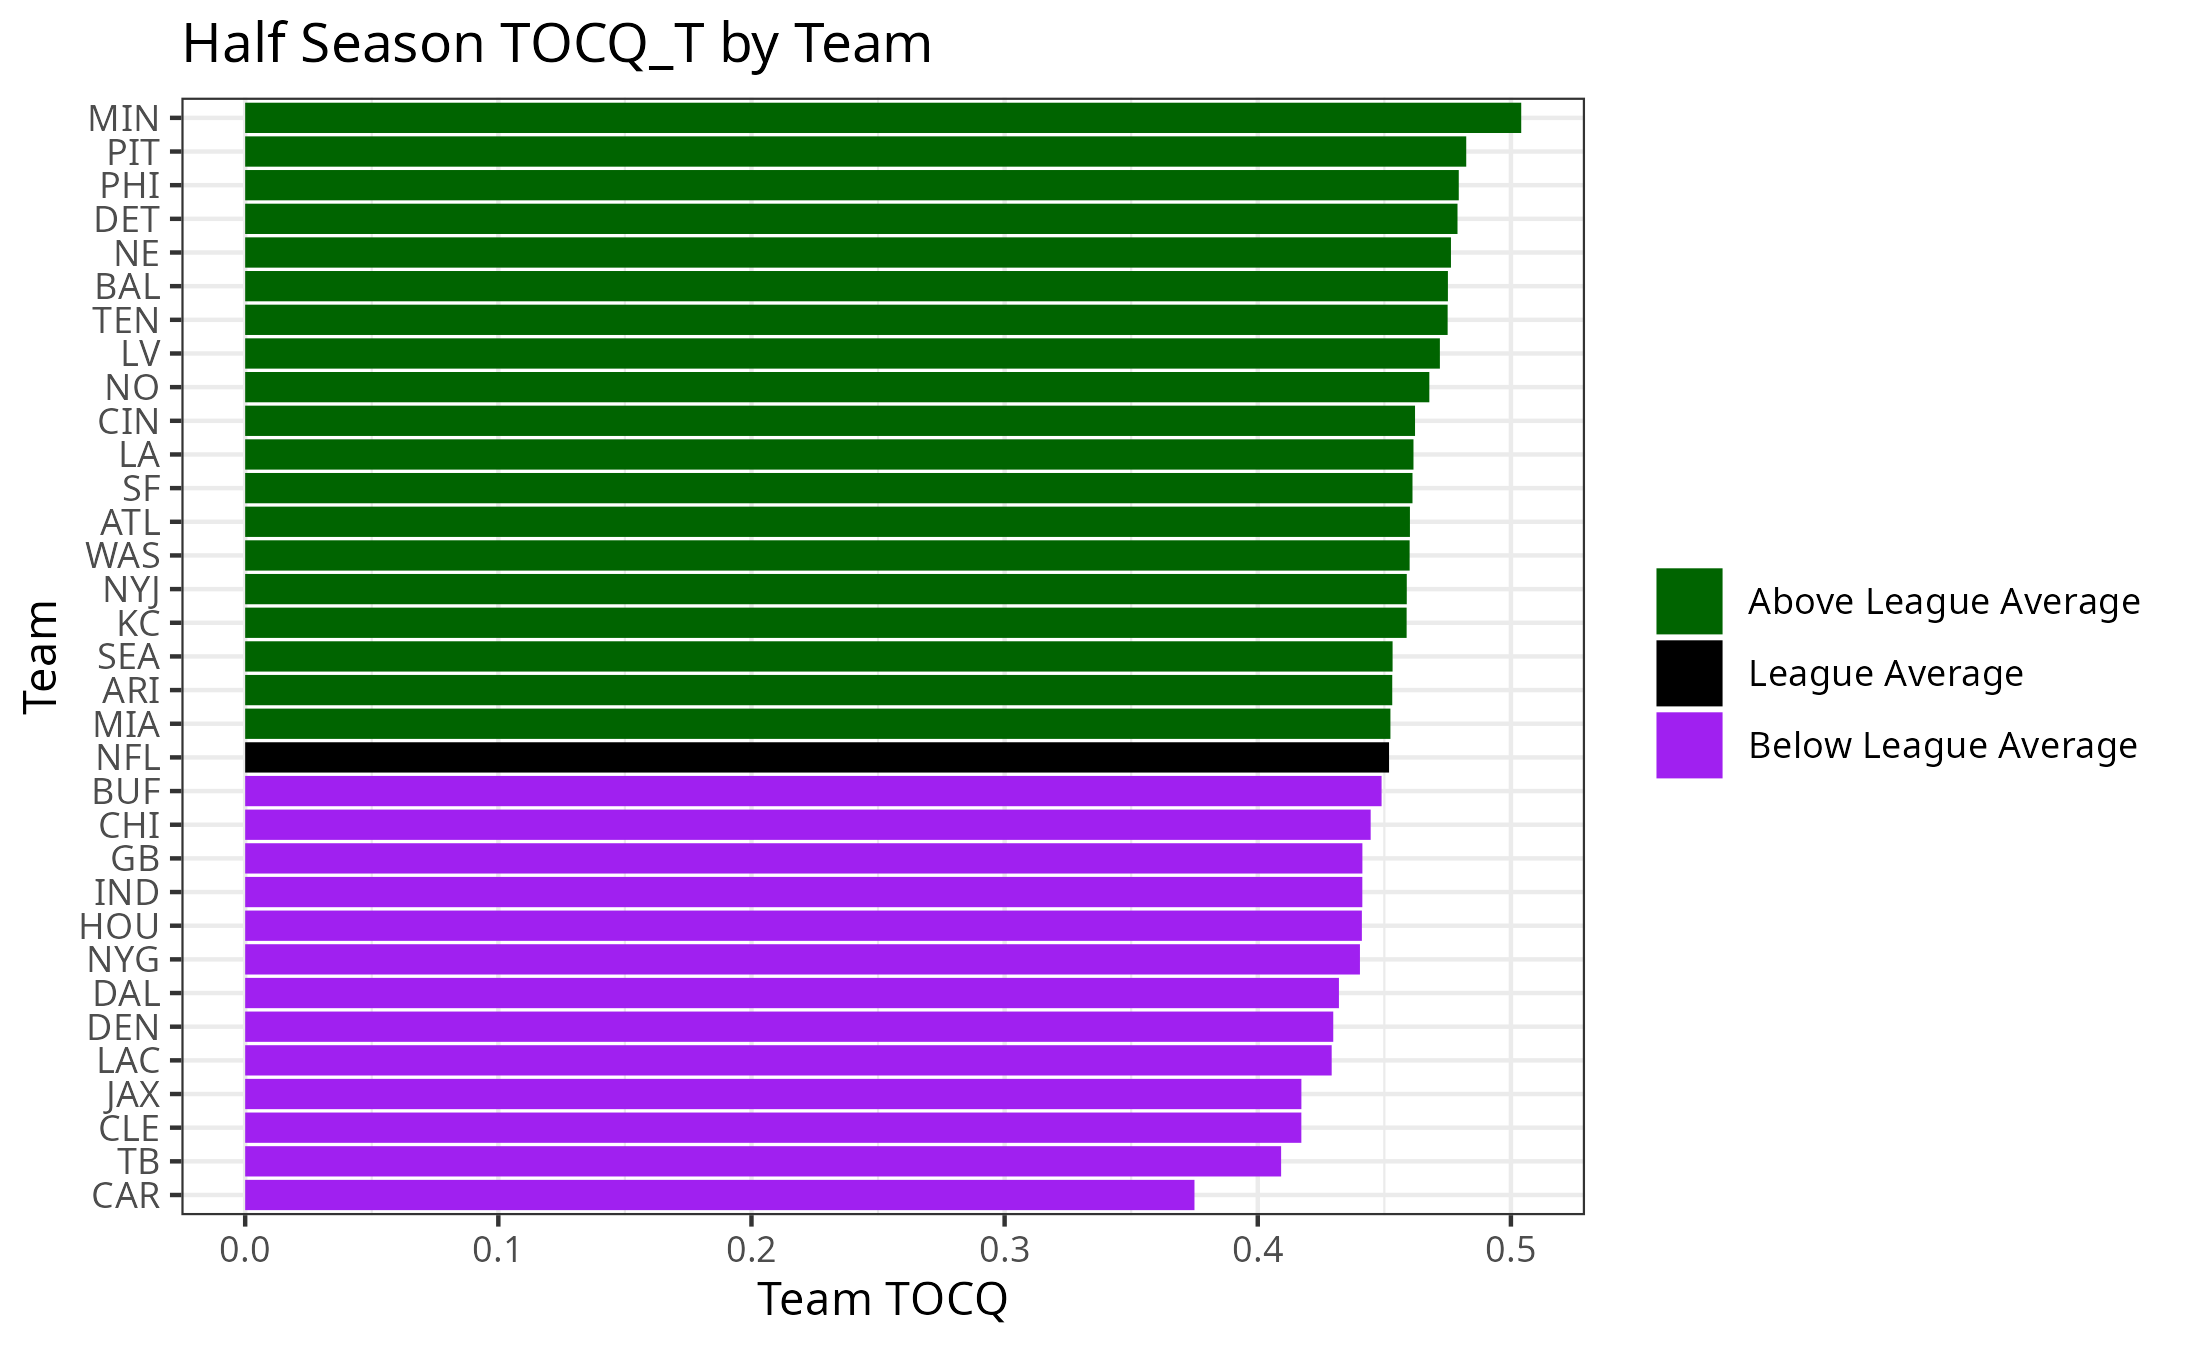
\includegraphics[width = \textwidth]{HalfSeasonTeam.png}
    \caption{Barplot of half-season \textbf{TOCQ$_T$} scores relative to league average.}
    \label{fig:HalfSeasonTeam}
\end{figure}

\begin{figure}[H]
    \centering
    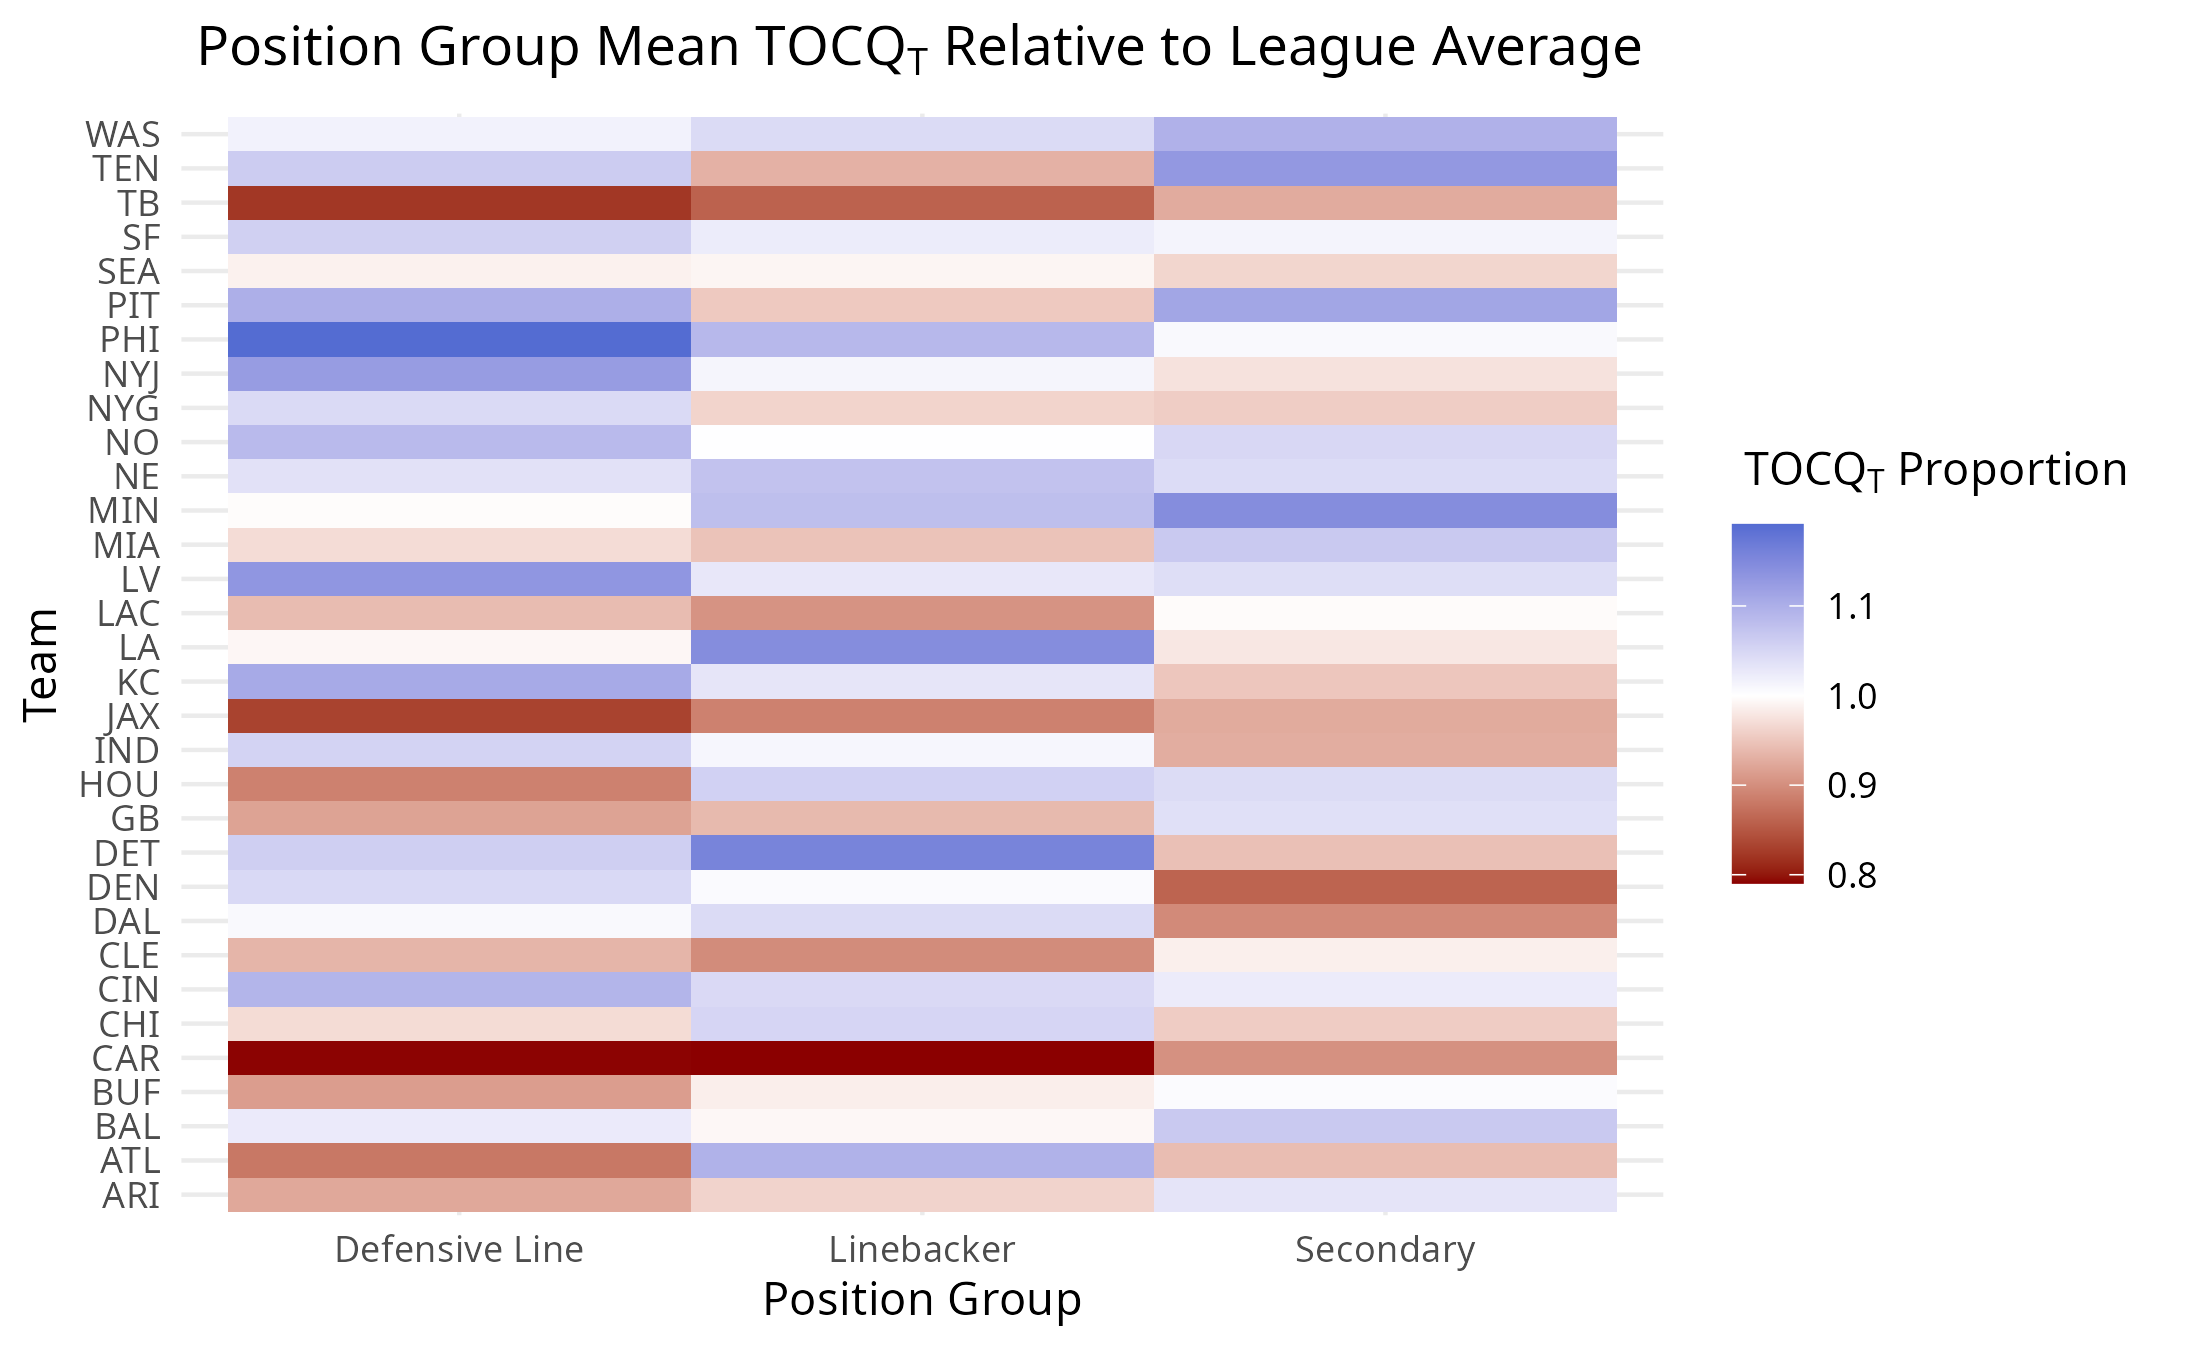
\includegraphics[width = \textwidth]{HalfSeasonTeamPositionGroup.png}
    \caption{Heatmap of half-season \textbf{TOCQ$_T$} scores broken down by position group, as a ratio relative to position group league average}
    \label{fig:HalfSeasonTeamPosGroup}
\end{figure}

\end{document}
